\begin{activity} \label{A:6.4.3}  In each of the following problems, determine the total force exerted by water against the surface that is described.
\begin{figure}[h]
\begin{center}
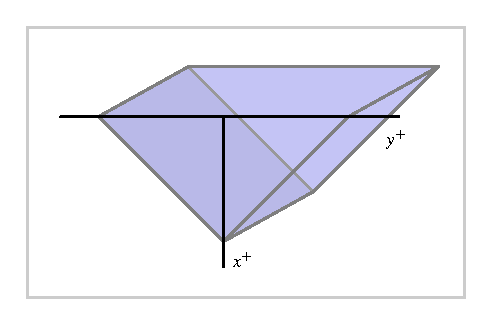
\includegraphics{figures/6_4_Act2Trough.eps}
\caption{A trough with triangular ends, as described in Activity~\ref{A:6.4.3}, part (c).} \label{F:6.4.Act3Trough}
\end{center}
\end{figure}
\ba
	\item Consider a rectangular dam that is 100 feet wide and 50 feet tall, and suppose that water presses against the dam all the way to the top.  
	\item Consider a semicircular dam with a radius of 30 feet.  Suppose that the water rises to within 10 feet of the top of the dam.
	\item Consider a trough with triangular ends, as pictured in Figure~\ref{F:6.4.Act3Trough}, where the tank is 10 feet long, the top is 5 feet wide, and the tank is 4 feet deep.  Say that the trough is full to within 1 foot of the top with water of weight density 62.4 pounds/ft$^3$.  How much force does the water exert against one of the triangular ends?
\ea

\end{activity}
\begin{smallhint}
\ba
	\item Small hints for each of the prompts above.
\ea
\end{smallhint}
\begin{bighint}
\ba
	\item Big hints for each of the prompts above.
\ea
\end{bighint}
\begin{activitySolution}
\ba
	\item Solutions for each of the prompts above.
\ea
\end{activitySolution}
\aftera